%% ------------------------------------------------------------------------- %%
\chapter{Test-Driven Development}
\label{cap:tdd}

Métodos ágeis de desenvolvimento de software focam sempre em constante
feedback, seja ele da equipe em relação ao cliente, ou da equipe em relação a
qualidade (interna e externa) do código produzido \cite{AgileManifesto}. Por
esse motivo, muitas das práticas sugeridas por métodos ágeis tentam aumentar o 
quantidade e a qualidade desse feedback; a ideia da programação pareada, por
exemplo, é dar retorno sobre o código durante sua escrita.

Test-Driven Development (TDD), popularizada por Kent Beck por meio de seu livro
\textit{TDD: By Example} em 2001 \cite{TDDByExample}, é mais uma das práticas
ágeis na qual o foco é dar feedback. TDD tem grande importância durante o ciclo
de desenvolvimento já que, conforme sugerido pelas práticas ágeis, o design de um
software deve emergir a medida que o software cresce. E, para responder
rapidamente a essas alterações, é necessário um constante feedback sobre a
qualidade interna e externa do código.

TDD é uma prática de desenvolvimento de software que é baseada na repetição de
um pequeno ciclo de atividades. Primeiramente, o desenvolvedor deve escrever um
teste que falha. Em seguida, deve fazer esse teste passar, implementando a
funcionalidade desejada. Por fim, deve refatorar o código. Esse ciclo,
exemplificado na figura \ref{fig:red-green-refactor} é também conhecido como 
Vermelho-Verde-Refatora (ou Red-Green-Refactor), já que lembram as cores que o 
desenvolvedor geralmente vê quando faz TDD: o vermelho geralmente significa que
o teste está falhando, e o verde quando o teste foi executado com sucesso.

\begin{figure}
  \centering
  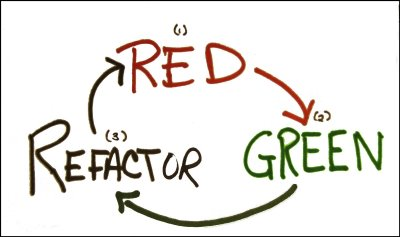
\includegraphics[scale=0.6]{ciclo-tdd}
  \caption{O ciclo Vermelho-Verde-Refatora}
  \label{fig:red-green-refactor}
\end{figure}

A velocidade que a prática dá retorno ao desenvolvedor possibilita que o mesmo
tome decisões sobre o código enquanto o custo de mudança ainda é
baixo. Segundo Vanderburg \cite{vanderburg}, TDD dá feedback em questão de
minutos, e só é inferior a da programação pareada. O gráfico,
baseado no trabalho dele, pode ser visto na Figura
\ref{fig:agile-feedback}.

\begin{figure}
  \centering
  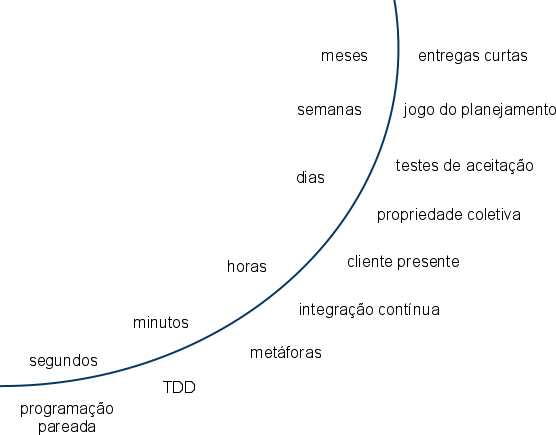
\includegraphics[scale=0.4]{agile-feedback-port}
  \caption{Práticas de XP e Tempo de Feedback (baseado em \cite{vanderburg})}
  \label{fig:agile-feedback}
\end{figure}

%% ------------------------------------------------------------------------- %%
\section{O ciclo}

Um desenvolvedor praticante de TDD escreve os testes antes do código de
produção. Beck define esse ciclo mais especificamente da seguinte maneira
\cite{TDDByExample} e reproduzido na Figura \ref{fig:passos-tdd}:

\begin{enumerate}
	\item Adicione o teste mais simples possível; 
	\item Rode todos os testes e veja o novo teste falhar; 
	\item Escreva o código mais simples que faça o teste passar; 
	\item Rode todos os testes e veja o novo teste passar; 
	\item Refatore para remover duplicação de dados e de código.
\end{enumerate}

Ao iniciar o ciclo, o programador deve escrever o próximo teste mais simples que
ela possa imaginar que falhe; em seguida, ele deve garantir que o teste que ele
escreveu realmente falha; com o teste falhando, o programador deve escrever o
código mais simples que ele possa escrever para fazer o código passar; em
seguida, ele deve checar que o teste que antes falhava, agora passa; por fim, o
programador deve refatorar todo o código duplicado que escreveu.

Simplicidade é algo intrínseco ao processo; o programador deve
buscar sempre escrever o teste mais simples que falhe e escrever o código mais simples
que faça o teste passar. Por fim, a última parte do ciclo é responsável por
tornar o código claro e flexível; nesse momento o programador deve
refatorar o código para remover toda a duplicação de dados ou de código gerada enquanto 
se preocupava em fazer o teste passar da maneira mais simples.

Em seu livro, Kent Beck \cite{TDDByExample} diz que o programador pode tomar
``passos de bebê'' (ou \textit{baby steps}) quando achar necessário. Esses
passos podem ser pequenos a ponto de fazer o programador implementar um método
simplesmente retornando uma constante, quanto maiores, fazendo o programador
implementar o algoritmo final. O programador deve usar sua experiência para
medir o tamanho do passo a ser dado, levando em conta sua confiança e
conhecimento da funcionalidade a ser implementada.

É possível ver que a prática divide o trabalho do desenvolvedor em duas partes.
A primeira se preocupa em escrever um código que funcione (composta pelas
atividades de escrever o teste e fazê-lo passar). Já a segunda parte se preocupa
com um código claro, expressivo e de fácil manutenção (composta pela atividade
de refatoração). Ron Jeffries fez uma famosa afirmação sobre TDD que explica
essa divisão: \textit{Código claro que funciona}. Na opinião dele, o programador 
primeiro se preocupa com a parte ``que funciona'', para depois deixar o ``código claro''.

\begin{figure}
  \centering
  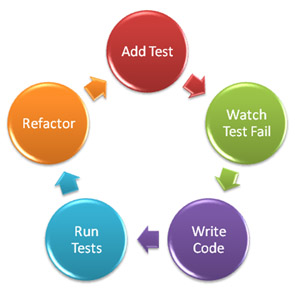
\includegraphics[scale=0.7]{passos-tdd}
  \caption{O ciclo detalhado de TDD.}
  \label{fig:passos-tdd}
\end{figure}

%% ------------------------------------------------------------------------- %%
\section{Benefícios da prática}

Uma consequência da prática de TDD é a bateria de testes de unidade gerada.
A mesma ajuda o programador a evitar erros de regressão, aonde a implementação de
uma nova funcionalidade quebra uma outra funcionalidade já existente no sistema.
Essa bateria também provê segurança durante as
constantes refatorações de código que são feitas durante o processo de
desenvolvimento, e permite com que ele altere o design e garanta que o
comportamento ainda é o mesmo. 
A cobertura de código coberto pelos testes também tende a ser alta, já que o
desenvolvedor deve sempre escrever um teste antes de implementar uma nova
funcionalidade. Além disso, por ser barato e rápido, a bateria é executada
muitas vezes ao dia, dando feedback constante ao programador.
Dave Astels \cite{astels-tdd} chama essa bateria
de testes de \textit{testes do programador}, já que ele é ferramenta de 
suporte ao trabalho do desenvolvedor.

A simplicidade agregada ao processo também é um dos benefícios da prática de
TDD. Os passos de bebê permitem ao desenvolvedor andar na velocidade que
sentir necessidade, indo mais rápido em partes mais triviais da implementação,
ou mais devagar em trechos mais complexos. Isso leva o desenvolvedor a escrever
códigos mais simples e fáceis de entender.

% TODO citar
Em projetos novos, praticantes de TDD afirmam que sentem menos necessidade da
utilização de recursos de depuração de código. A quantidade de código
escrita entre um teste e outro tende a ser pequena, e caso um teste falhe
inesperadamente, o programador pode simplesmente reverter as alterações para a 
versão anterior estável e começar novamente. Essa abordagem pode muitas vezes
ser mais produtiva do que a atividade de depuração \cite{janzen-arch-improvement}.
Por essas e outras razões, desenvolvedores afirmam que são mais produtivos
quando praticam TDD. Apesar do custo da escrita do teste existir, à longo prazo
o desenvolvedor gasta menos tempo com depurações ou erros de regressão (citar).
